One of the major motivations for the development of \libpnicore\ was the lack of
native support for multidimensional (MD) arrays in C++. This section goes into
details how such arrays are implemented in \libpnicore. Thus this part of the
documentation is intended for developers and those who want to know more about
the internals of \libpnicore. 

The classical approach towards MD arrays in C/C++ would be to do something like
this
\begin{minted}{cpp}
double matrix[3][3];
\end{minted}
However, this approach has a whole bunch of problems
\begin{enumerate}
\item the variable {\tt matrix} is allocated on the stack which will cause
problems if the matrix becomes large
\item there is no easy way how to allocate such a variable on the heap (at least
not at runtime)
\item there is no native support for arithmetic operations on multidimensional
arrays 
\item there is no native support for slicing (select a sub region) of such
arrays.
\end{enumerate}
There is a language that has perfect support for MD arrays: Fortran. In the
standards Fortran 90 and higher the language shows all the features required to
easily work with MD arrays. It is thus not surprising that Fortran was an
inspiration for the design of the MD array interface in \libpnicore. 
There is still one question left: if Fortran is so superior with MD arrays, why
not write the numerical part of the software in Fortran and everything else in
C++? The reason is simple: while Fortran is quite good for writing short and
rather straight forward numerical applications, its lack of a standard library
providing higher level data structures such as lists or maps render it
inconvenient for the implementation of large software systems. In addition, its
lack of {\em generics} or {\em template} support requires a user to reimplement
an algorithm for each desired data type which is obviously horribly inefficient. 
C++ offers all the tools for implementing a fast and easy to use MD array
interface whose performance can compete with those of Fortran as will be shown
later. 

\section{Basic concepts of multidimensional arrays}

Before we continue with the technical description of how MD arrays are
implemented we first need to define some terminology 
\begin{description}
\item[rank] the number of dimensions of an MD array, typically abbreviated with
$r$
\item[elements per dimension] the number of elements along each dimension is
denoted by $n_i$ where $i=1,\hdots,r$.
\item[total number of elements] denoted by $n_{\mathrm{tot}}$ is the total
number of elements stored in a MD array and can be computed with 
\begin{align}
    n_{\mathrm{tot}} = \prod_{i=1}^r n_i
\end{align}
\item[element type] the data type of the elements stored in the array,
abbreviated with {\tt ETYPE}. 
\end{description}

%%-----------------------------------------------------------------------------
\begin{figure}[tb]
\centering
\begin{minipage}[c]{0.55\linewidth}
\centering
\resizebox{\linewidth}{!}{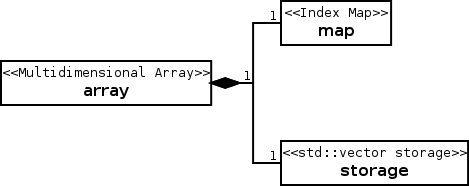
\includegraphics{pics/md_array_basic_structure.png}}
\end{minipage}
\hfill
\begin{minipage}[c]{0.39\linewidth}
\caption{{\small\label{fig:array_app:basic_structure} A MD array consists of a
storage and an index map. The former holds all the data elements in memory while
the latter one maps multidimensional indexes uniquely to linear offsets in the
storage.
}}
%%-----------------------------------------------------------------------------
\end{minipage}
\end{figure}
To overcome the issues that classical MD arrays have in C or C++ we need a more
elaborate data structure to describe the array. In \libpnicore\ a MD array
consists of two components (see also Fig.~\ref{fig:array_app:basic_structure})
\begin{enumerate}
\item a linear storage of size $n_{\mathrm{tot}}$ for elements of type {\tt
ETYPE}
\item a so called index map {\tt IMAP} which is a data structure providing a
unique mapping between a multidimensional index $(i,j,k,\hdots)$ and a linear
offset in the storage. 
\end{enumerate}
The storage can be any data structure that can hold elements of type {\tt ETYPE}
contiguously in memory and exposes an interface compatible to that of {\tt std::vector}.

\section{Index maps}

%%%----------------------------------------------------------------------------
\begin{figure}[tb]
\centering
\begin{minipage}{0.3\linewidth}
\centering
\resizebox{\linewidth}{!}{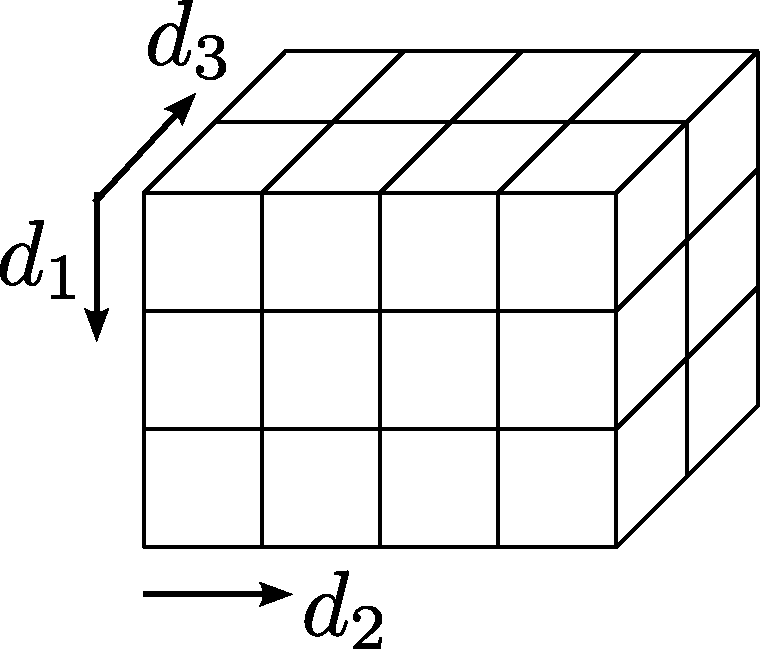
\includegraphics{pics/array_3d.pdf}}
\end{minipage}
\hfill
\begin{minipage}{0.45\linewidth}
\caption{{\small\label{fig:array_app:array_3d}
The 3-dimensional array of shape $(3,4,2)$ which will be used for all following
examples. 
}}
\end{minipage}
\end{figure}
%%%----------------------------------------------------------------------------
Index maps serve two purposes 
\begin{enumerate}
\item compute the linear offset for a given multidimensional index
\item compute the multidimensional index for a given offset.
\end{enumerate}
It is indeed the implementation of the index map which determines whether or not
an array is in row- or column-major ordering (see also
sections~\ref{sec:c_ordering} and \ref{sec:f_ordering} for details on this).
In particular the first procedure is the core of all MD array implementation.
When an element of a MD array is addressed by a multidimensional index
$(i,j,k,\hdots)$ this index must be converted (uniquely) to a linear offset in
the storage. There are currently two standard schemas how MD indexes are mapped
to linear memory
\begin{itemize}
\item row-major ordering (this is how all C-like languages are doing it)
\item and column-major ordering (the Fortran way).
\end{itemize}
In more general terms the question reads: which index varies fastest or which
index is contiguous in memory. In row-major this is true for the last index
while for column-major ordering the first index is contiguous in memory.
These two cases will be now discussed in more detail.

For all further considerations we will use an example as depicted in
Fig.~\ref{fig:array_app:array_3d} which is a 3 dimensional array of arbitrary
element type and shape $(3,4,2)$.

\subsection{Row major- or C-ordering}\label{sec:c_ordering}

%%-----------------------------------------------------------------------------
\begin{figure}[tb]
\centering
\begin{minipage}{0.45\linewidth}
\centering
\resizebox{\linewidth}{!}{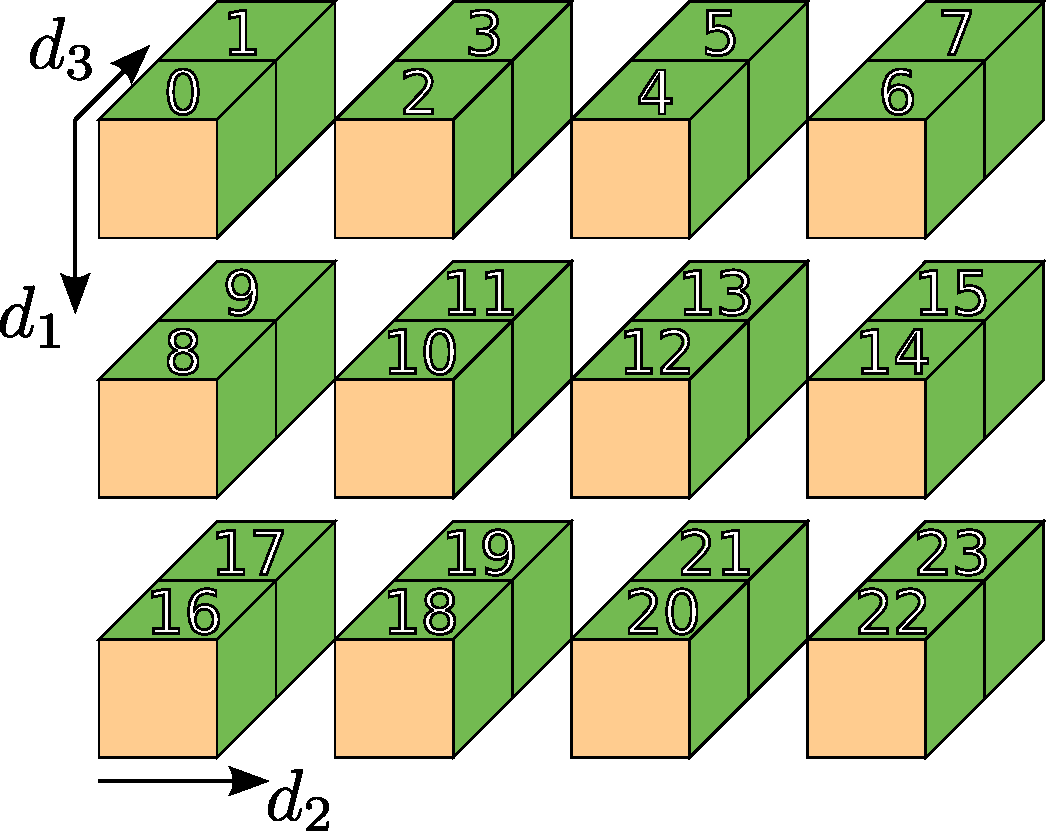
\includegraphics{pics/array_3d_corder.pdf}}
\end{minipage}
\hfill
\begin{minipage}{0.4\linewidth}
\caption{{\small\label{fig:array_app:array_3d_corder}
The array shown in Fig.~\ref{fig:array_app:array_3d} in C-ordering (row major
ordering). The last index varies fastest and is thus contiguous in memory. 
}}
\end{minipage}
\end{figure}
%%-----------------------------------------------------------------------------
Row major ordering is the standard layout in memory for multidimensional array
sin C and most other languages derived from it. In this case the last index
varies fastest and is thus contiguous in memory as shown in
Fig.~\ref{fig:array_app:array_3d_corder}. 
The transformation of the MD index $\mathbf{i}=(i,j,k)$ to the linear offset 
$o$ can be written as a scalar product 
\begin{align}\label{eq:array_app:offset_formula}
    o = \mathbf{s}\mathbf{i}
\end{align}
where $\mathbf{s}$ denotes the stride vector whose elements are given with
\begin{align}
    s_i &= \prod_{j=i+1}^r n_j \\
    s_r &= 1
\end{align}
For the above example the stride vector would read $\mathbf{s}=(8,2,1)$. 
The other direction, computing the index from a given offset is a bit more
difficult. 

\subsection{Column major- or Fortran-ordering}\label{sec:f_ordering}
%%-----------------------------------------------------------------------------
\begin{figure}[tb]
\centering
\begin{minipage}{0.5\linewidth}
\centering
\resizebox{\linewidth}{!}{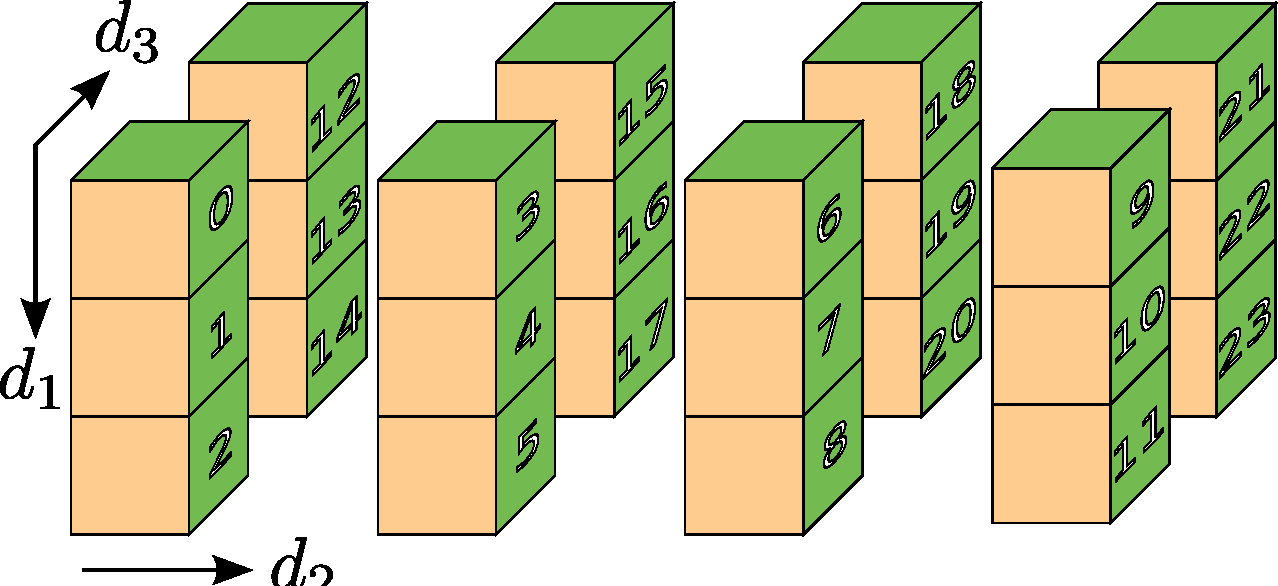
\includegraphics{pics/array_3d_forder.pdf}}
\end{minipage}
\hfill
\begin{minipage}{0.4\linewidth}
\caption{{\small\label{fig:array_app:array_3d_forder}
The array shown in Fig.~\ref{fig:array_app:array_3d} in Fortran-ordering (column major
ordering). The first index varies fastest and is thus contiguous in memory. 
}}
\end{minipage}
\end{figure}
%%-----------------------------------------------------------------------------
This schema for data organization is commonly used in languages like Fortran,
Pascal, or Ada. The layout of data elements in memory for our example array is
shown in Fig.~\ref{fig:array_app:array_3d_forder}. The formula for the offset
calculation is the same as for C-ordering and can be found  in
Eq.~(\ref{eq:array_app:offset_formula}). What is different here is the stride
vector. The algorithm to compute its elements reads
\begin{align}
    s_0 &= 1 \\
    s_i &= \prod_{j=0}^in_j
\end{align}

\subsection{Arbitrary ordering}\label{sec:a_ordering}
%%-----------------------------------------------------------------------------
\begin{figure}[tb]
\centering
\begin{minipage}{0.35\linewidth}
\centering
\resizebox{\linewidth}{!}{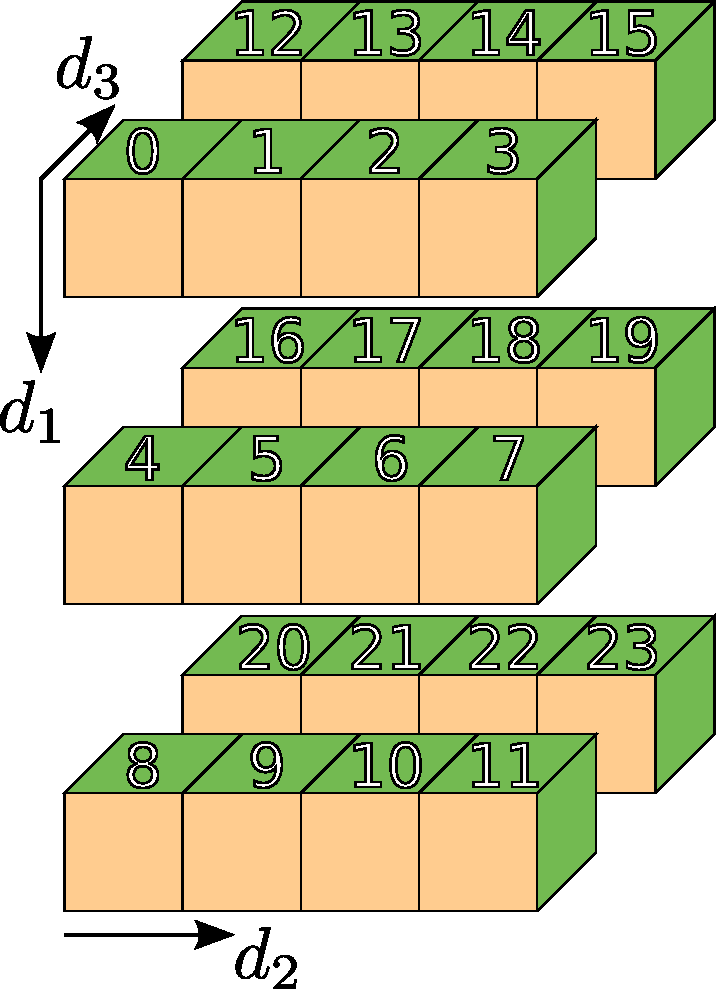
\includegraphics{pics/array_3d_aorder.pdf}}
\end{minipage}
\hfill
\begin{minipage}{0.4\linewidth}
\caption{{\small\label{fig:array_app:array_3d_aorder}
The array shown in Fig.~\ref{fig:array_app:array_3d} using an arbitrary ordering
scheme where the second index varies fastest, followed by the first and the
last.
}}
\end{minipage}
\end{figure}
%%-----------------------------------------------------------------------------

\subsection{The basic interface}

\begin{minted}{cpp}
class index_map
{
    public:
    //======================public types========================
    typedef .... const_iterator;

    //======================public methods======================
    index_map();                  //default constructible
    index_map(const index_map &); //copy constructible 

    index_map &operator=(const index_map &s); //copy assignable 

    //compute offset from a varidic list of indexes
    template<typename ...ITYPES> size_t offset(ITYPES ...indices);

    //compute offset from a container type
    template<CTYPE> size_t offset(const CTYPE &v);

    //compute index from a given offset
    template<CTYPE> CTYPE index(size_t offset);

    size_t rank() const;  //get number of dimensions
    size_t size() const;  //get number of dimensions
    
    const_iterator begin() const; 
    const_iterator end() const; 

};
\end{minted}

\section{Selections}

\section{Array arithmetics}

\section{Performance considerations}

